\chapter{WORKSPACE}
\section{Topic}
Give a comment on the workspace.
\section{Theory}
Existing of any solution raises the question of the manipulator's workspace, which is the volume of space that the end-effector of the manipulator can reach.
\section{Application}
We have: 
\[
\left\{
\begin{aligned}
x &= \ell_4 \cdot \cos(\theta_1 + \theta_4) + \ell_3 \cdot \cos\theta_1 \\
y &= \ell_4 \cdot \sin(\theta_1 + \theta_4) + \ell_3 \cdot \sin\theta_1 \\
z &= d_2
\end{aligned}
\right.
\]
With:
\begin{itemize}
    \item $\ell_3 = 1000\,\text{mm}$
    \item $\ell_4 = 300\,\text{mm}$
    \item $d_2 \in [2150; 2750]$
    \item $\theta_1 \in [0^\circ; 360^\circ]$
    \item $\theta_4 \in [-90^\circ; 90^\circ]$
\end{itemize}
Next:
\[
    x^2 + y^2 = \ell_4^2 + \ell_3^2 + 2\ell_3 \ell_4 \cos(\theta_4)
\]
\[
    \Leftrightarrow \cos(\theta_4) = \frac{x^2 + y^2 - \ell_4^2 - \ell_3^2}{2 \ell_3 \ell_4}
\]
We also have:
\[
    0 \leq \cos(\theta_4) \leq 1
\]
\[
    \Rightarrow 0 \leq x^2 + y^2 \leq (\ell_4 + \ell_3)^2
\]
\[
\Rightarrow 
\left\{
\begin{aligned}
0 &\leq x^2 + y^2 \leq 1690000 \\
d_2 &\in [2150; 2750] \\
\theta_1 &\in [0^\circ; 360^\circ] \\
\theta_4 &\in [-90^\circ; 90^\circ]
\end{aligned}
\right.
\]
To simplify matters, we remove the mechanical constraint, the joints can be fully rotated. Therefore, our workspace is idealized.
\begin{figure}[H]
    \centering
    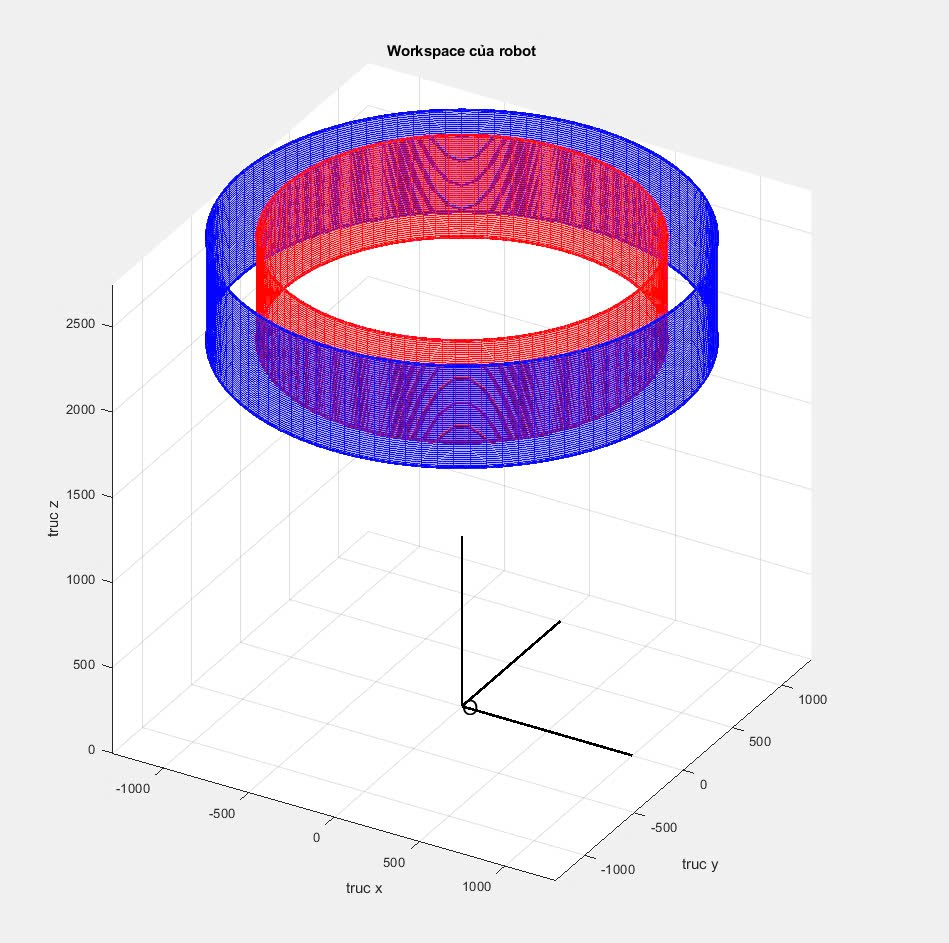
\includegraphics[width=0.5\textwidth]{pictures/workspace1.png} 
    \caption{Workspace of the robot}
\end{figure}
\begin{figure}[H]
    \centering
    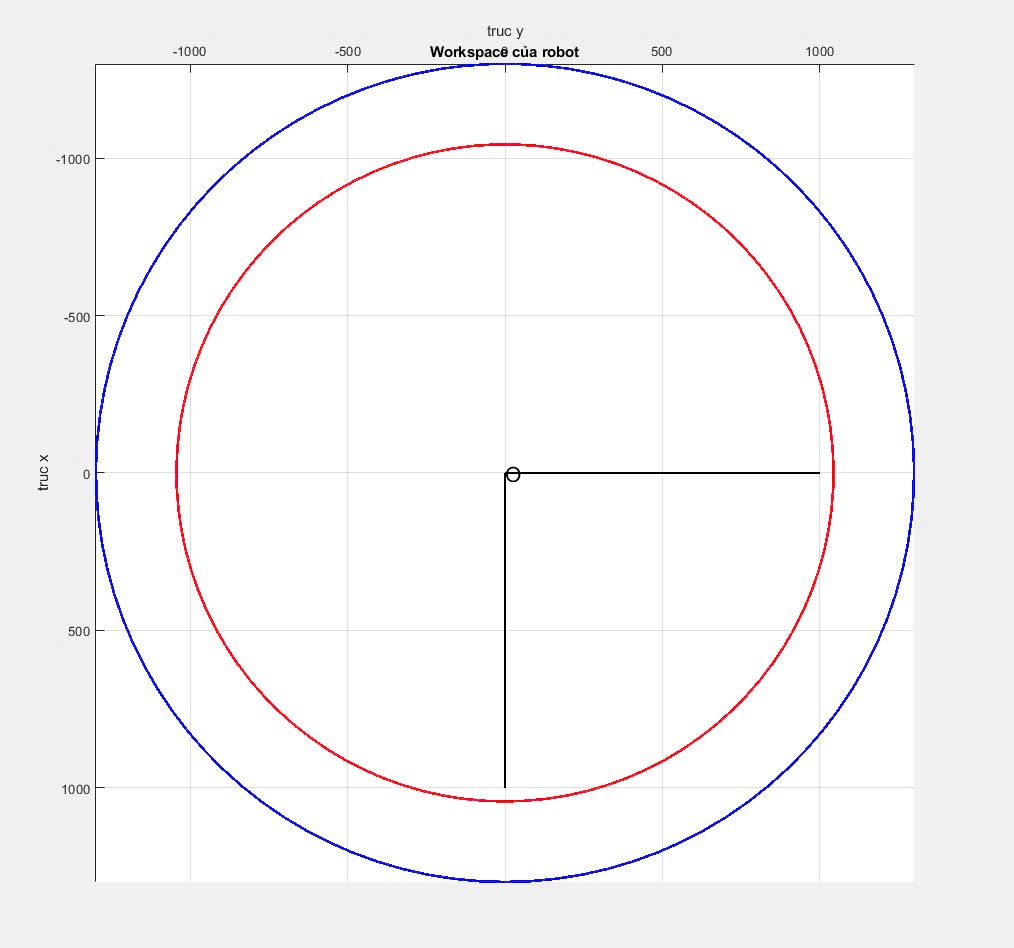
\includegraphics[width=0.5\textwidth]{pictures/workspace2.png} 
    \caption{Workspace of the robot another view}
\end{figure}
\chapter{JACOBIAN MATRIX}
\section{Topic}
Formulate the Jacobian matrix for this robot. Is there any singularity?
\section{Theory}
The Jacobian is a multidimensional form of the derivative. The 6 x 6 matrix of partial derivatives is the Jacobian $J$, as mapping velocities in $X$ to those in $Y$. \\
In the field of robotics, Jacobians are used to relate joint velocities to Cartesian velocities of the tip of the arm.

\[
{}^0\mathbf{V} = {}^0\!J(\theta) \, \dot{\theta}
\]

All manipulators have singularities at:
\begin{itemize}
    \item The boundary of their workspace.
    \item Most have loci of singularities inside their workspace.
\end{itemize}
\section{Application}
Vector of joint variables:
\[
\mathbf{Q} = \begin{bmatrix} \theta_1 & d_2 & \theta_4 \end{bmatrix}^T
\]
Position-orientation state vector $\mathbf{X}$:
\[
\mathbf{X} = \begin{bmatrix} p_x & p_y & d_2 & 0 & 0 & \theta_1 + \theta_4 \end{bmatrix}^T
\]
\[
= \begin{bmatrix} 
\ell_4 \cos(\theta_1 + \theta_4) + \ell_3 \cos \theta_1 & 
\ell_4 \sin(\theta_1 + \theta_4) + \ell_3 \sin \theta_1 & 
d_2 & 
0 & 
0 & 
\theta_1 + \theta_4 
\end{bmatrix}^T
\]
The Jacobian matrix $J$ is the partial derivative of the position vector $\mathbf{X}$ with respect to the joint variable vector $\mathbf{q}$:

\[
J = \frac{\partial \mathbf{X}}{\partial \mathbf{q}} =
\begin{bmatrix}
\frac{\partial p_x}{\partial \theta_1} & \frac{\partial p_x}{\partial d_2} & \frac{\partial p_x}{\partial \theta_4} \\
\frac{\partial p_y}{\partial \theta_1} & \frac{\partial p_y}{\partial d_2} & \frac{\partial p_y}{\partial \theta_4} \\
\frac{\partial d_2}{\partial \theta_1} & \frac{\partial d_2}{\partial d_2} & \frac{\partial d_2}{\partial \theta_4} \\
0 & 0 & 0 \\
0 & 0 & 0 \\
\frac{\partial (\theta_1 + \theta_4)}{\partial \theta_1} & \frac{\partial (\theta_1 + \theta_4)}{\partial d_2} & \frac{\partial (\theta_1 + \theta_4)}{\partial \theta_4}
\end{bmatrix}
\]

\[
=
\begin{bmatrix}
-\ell_4 \sin(\theta_1 + \theta_4) - \ell_3 \sin\theta_1 & 0 & -\ell_4 \sin(\theta_1 + \theta_4) \\
\ell_4 \cos(\theta_1 + \theta_4) + \ell_3 \cos\theta_1 & 0 & \ell_4 \cos(\theta_1 + \theta_4) \\
0 & 1 & 0 \\
0 & 0 & 0 \\
0 & 0 & 0 \\
1 & 0 & 1
\end{bmatrix}
\]
\[
\Rightarrow \text{ Control matrix } \mathbf{J} = 
\begin{bmatrix}
-\ell_4 \sin(\theta_1 + \theta_4) - \ell_3 \sin \theta_1 & 0 & -\ell_4 \sin(\theta_1 + \theta_4) \\
\ell_4 \cos(\theta_1 + \theta_4) + \ell_3 \cos \theta_1 & 0 & \ell_4 \cos(\theta_1 + \theta_4) \\
0 & 1 & 0
\end{bmatrix}
\]
\textbf{Case of Jacobian Singularity}
\[
J = \begin{bmatrix}
-l_4 \sin(\theta_0 + \theta_4) & -l_3 \sin\theta_1 & 0 & -l_4 \sin(\theta_1 + \theta_4) \\
l_4 \cos(\theta_0 + \theta_4) + l_3 \cos\theta_1 & 0 & 0 & l_4 \cos(\theta_1 + \theta_4) \\
0 & 1 & 0 & 0 \\
0 & 0 & 1 & 0
\end{bmatrix}
\]

\[
\det(J_a) = a_{11} \cdot (a_{22} \cdot a_{33} - a_{23} \cdot a_{32}) - a_{12} \cdot (a_{21} \cdot a_{33} - a_{23} \cdot a_{31}) + a_{13} \cdot (a_{21} \cdot a_{32} - a_{22} \cdot a_{31})
\]
\[
= [-l_4 \sin(\theta_0 + \theta_4) - l_3 \sin\theta_1][l_4 \cos(\theta_1 + \theta_4)] + [-l_4 \sin(\theta_1 + \theta_4)][l_4 \cos(\theta_0 + \theta_4) + l_3 \cos\theta_1]
\]
\[
-l_4^2 \sin(\theta_0 + \theta_4) \cos(\theta_1 + \theta_4) + l_3 \sin\theta_1 l_4 \cos(\theta_1 + \theta_4) - l_4^2 \sin(\theta_1 + \theta_4)\cos(\theta_0 + \theta_4) 
\]
\[
- l_3 l_4 \sin(\theta_1 + \theta_4)\cos\theta_1
\]

\[
= l_3 l_4 [\sin\theta_1 \cdot \cos(\theta_1 + \theta_4) - l_4 l_3 \sin(\theta_1 + \theta_4) \cdot \cos\theta_1]
\]

\[
= -l_3 \cdot l_4 \cdot \sin(-\theta_4)
\]

\[
\det(J_a) = 0 \iff -l_4 \cdot l_3 \cdot \sin(-\theta_4) = 0
\]

\[
\iff -l_3 \cdot l_4 \cdot \sin(\theta_4) = 0
\]

\[
\iff \theta_4 = k\pi (k \in \mathbb{Z}); \theta_4 \in [-90^\circ, 90^\circ]
\]

\[
\Rightarrow \text{The point is within the range where } \theta_4 = 0
\]